%!TEX root = karen.tex

These figures represent optimizations of the Cosine Bell and Vortex Roll-up test cases. Essentially, the optimizations here are general for multi-GPU SpMV. Improving these test cases improves all explicit schemes for RBF-FD (i.e., hyperbolic and parabolic equations, and various time stepping schemes like euler, RK4, Adams-Bashforth etc.). 


For the MPI I might need to have multiple figures comparing performance. However, for the GPU optimizations I can show a single plot with all the curves on it. These sections will be good 

\section{MPI\_Alltoallv}
Change send/recv to alltoallv. Track wait time. Show limitation on scalability with GPU (sublinear) vs CPU (linear). How high can we get linear on CPU? 


Communication between processors requires each processor to iterate through their neighboring processors and share information. This can be seen as a simple for loop allowing every processor to touch its neighbors in round-robin fashion. The benchmarks seen in \authnote{figures from paper1} show the strong scaling of our implementation with a for loop and send/recv. 

In Figs~\ref{figs:alltoall_scaling} we show the strong scaling of the cosine bell after 

Alternatively

an all to all collective. That is, all processors share some information with potentially every other processor. 

\authnote{cleanup:} 
These results were run on Keeneland. The changes to MPI communication are the result of changing from blocking communication (MPI\_send/MPI\_recv) to non-blocking communication (MPI\_alltoall).

\begin{figure}[htbp]
\centering
\begin{subfigure}[b]{0.425\textwidth}
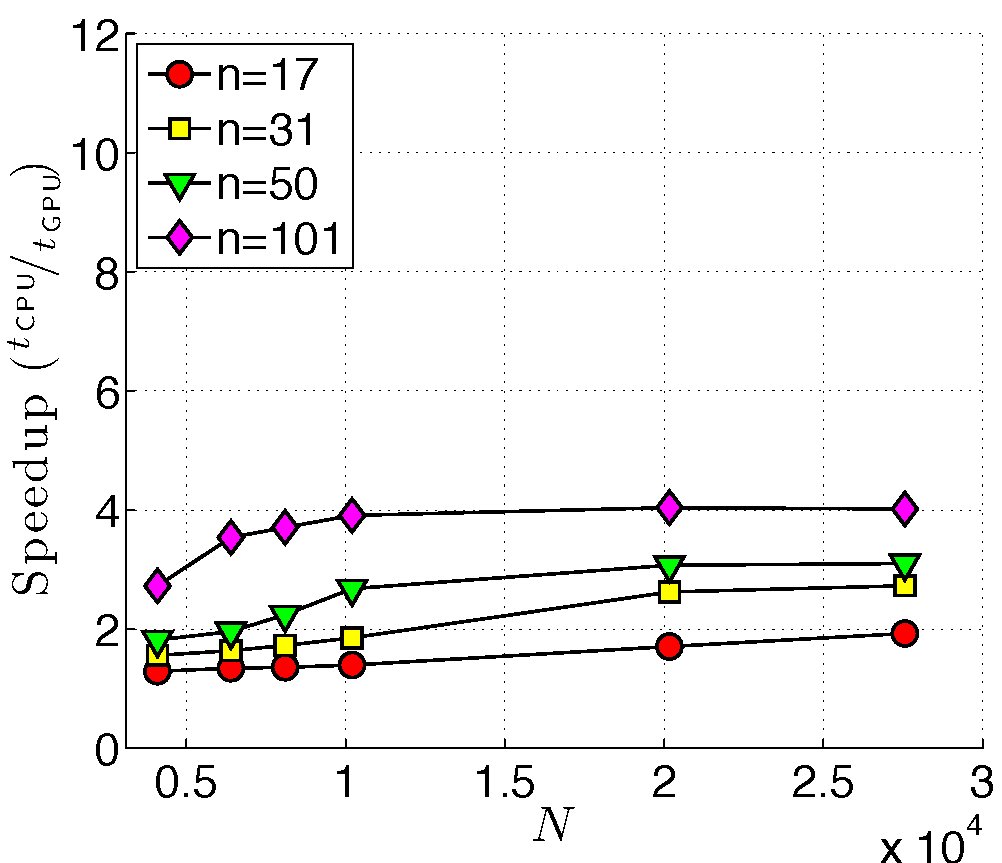
\includegraphics[width=1.0\textwidth]{../figures/chapter5/alltoallv/speedup_1proc_oneWarpPerStencil.pdf}
\caption{One warp per stencil kernel on one GPU in Keeneland}
\label{fig:alltoall_1proc_warp}
\end{subfigure} 
\begin{subfigure}[b]{0.425\textwidth}
\centering
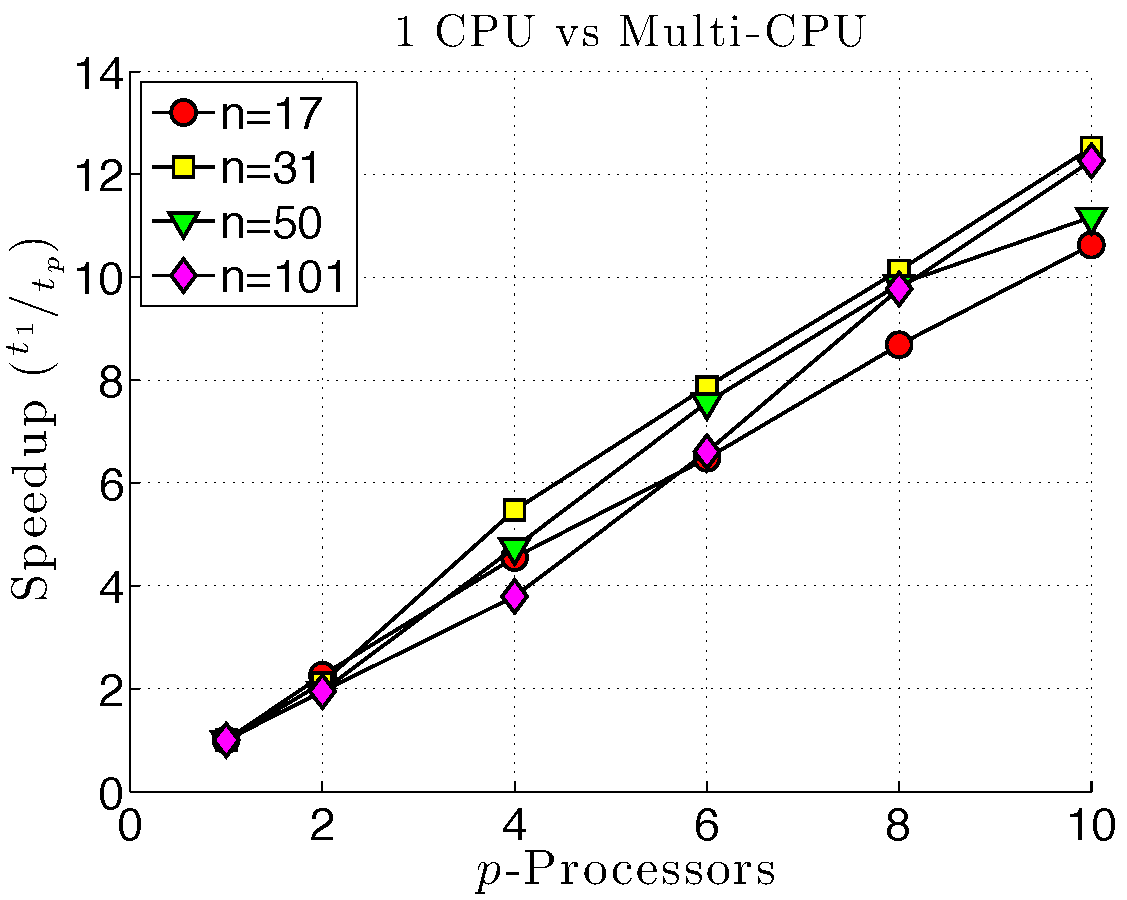
\includegraphics[width=1.0\textwidth]{../figures/chapter5/alltoallv/speedup_1CPU_vs_NCPU.pdf}
\caption{Multi-CPU strong scaling on Keeneland for one warp per stencil}
\label{fig:alltoall_multicpu_scaling}
\end{subfigure} 
\begin{subfigure}[b]{0.425\textwidth}
\centering
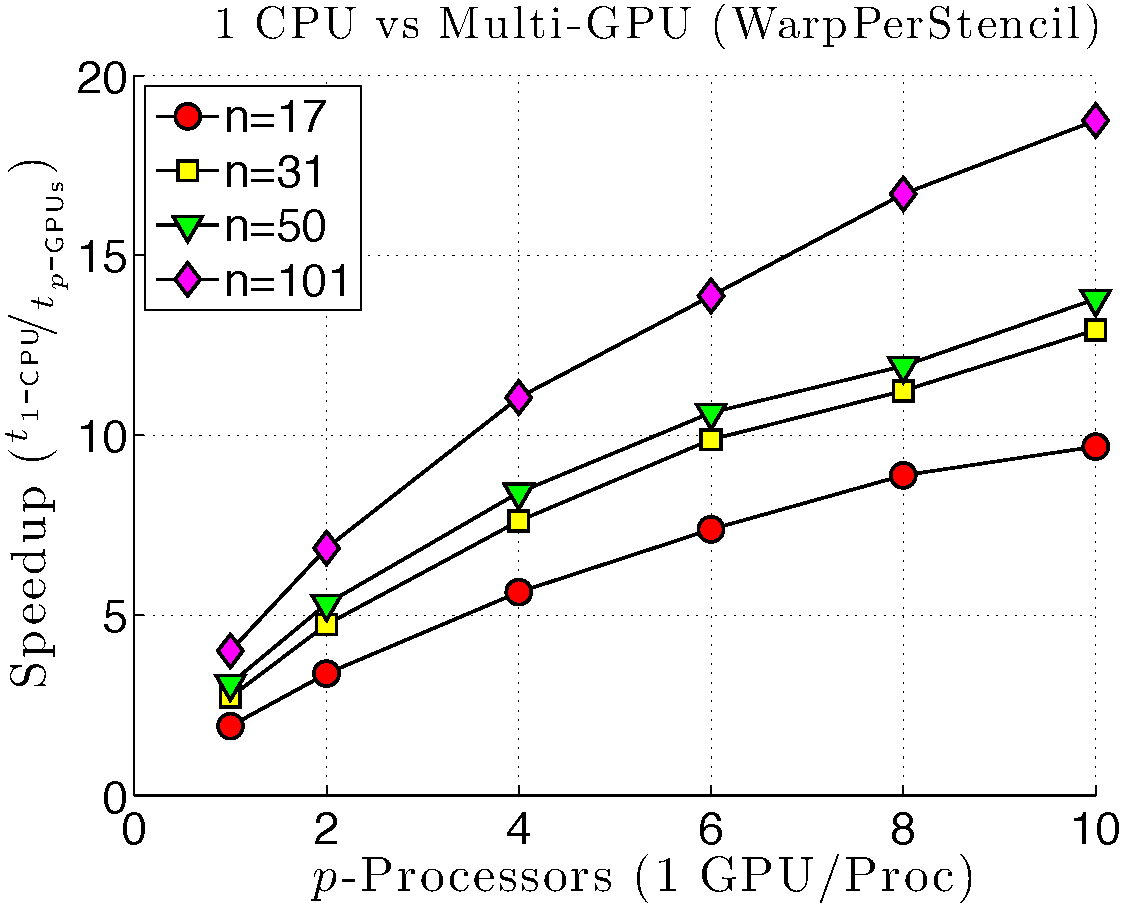
\includegraphics[width=1.0\textwidth]{../figures/chapter5/alltoallv/speedup_1CPU_vs_NGPU_WarpPerStencil.pdf}
\caption{Multi-GPU strong scaling vs one CPU on Keeneland for one warp per stencil}
\label{fig:alltoall_multigpu_vs_cpu_scaling}
\end{subfigure} 
\begin{subfigure}[b]{0.425\textwidth}
\centering
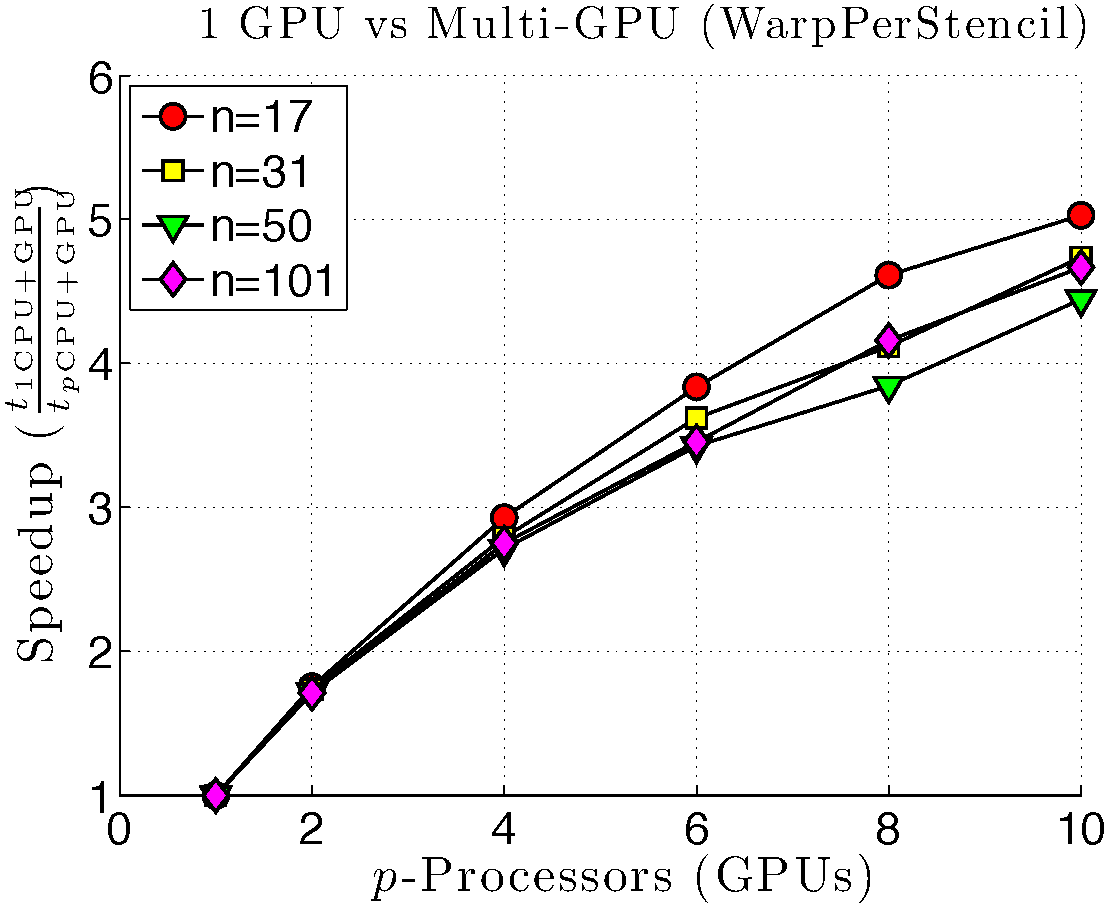
\includegraphics[width=1.0\textwidth]{../figures/chapter5/alltoallv/speedup_1GPU_vs_NGPU_WarpPerStencil.pdf}
\caption{Multi-GPU strong scaling vs one GPU on Keeneland for one warp per stencil}
\label{fig:alltoall_multigpu_vs_gpu_scaling}
\end{subfigure} 
\begin{subfigure}[b]{0.425\textwidth}
\centering
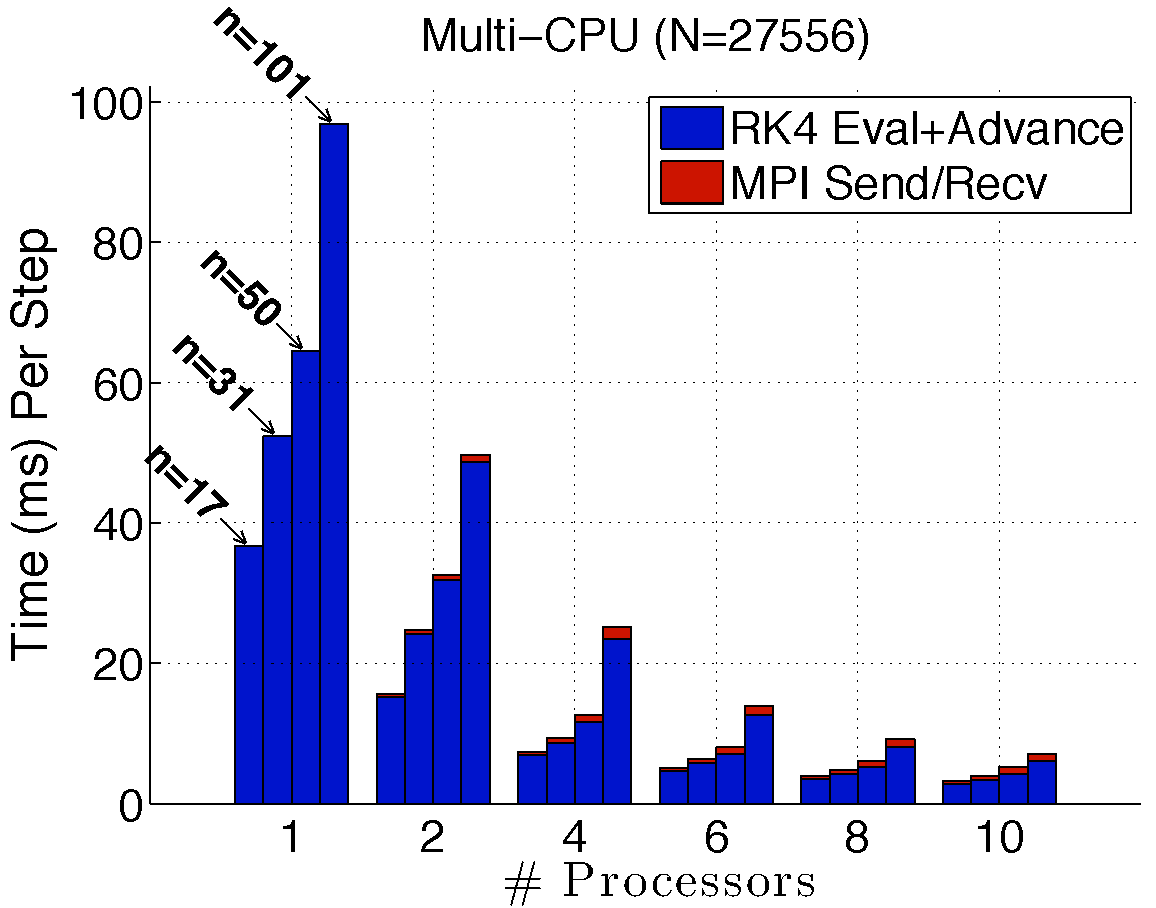
\includegraphics[width=1.0\textwidth]{../figures/chapter5/alltoallv/multiCPU_costs.pdf}
\caption{Multi-CPU benchmarks by component on Keeneland}
\label{fig:alltoall_multicpu_costs}
\end{subfigure} 
\begin{subfigure}[b]{0.425\textwidth}
\centering
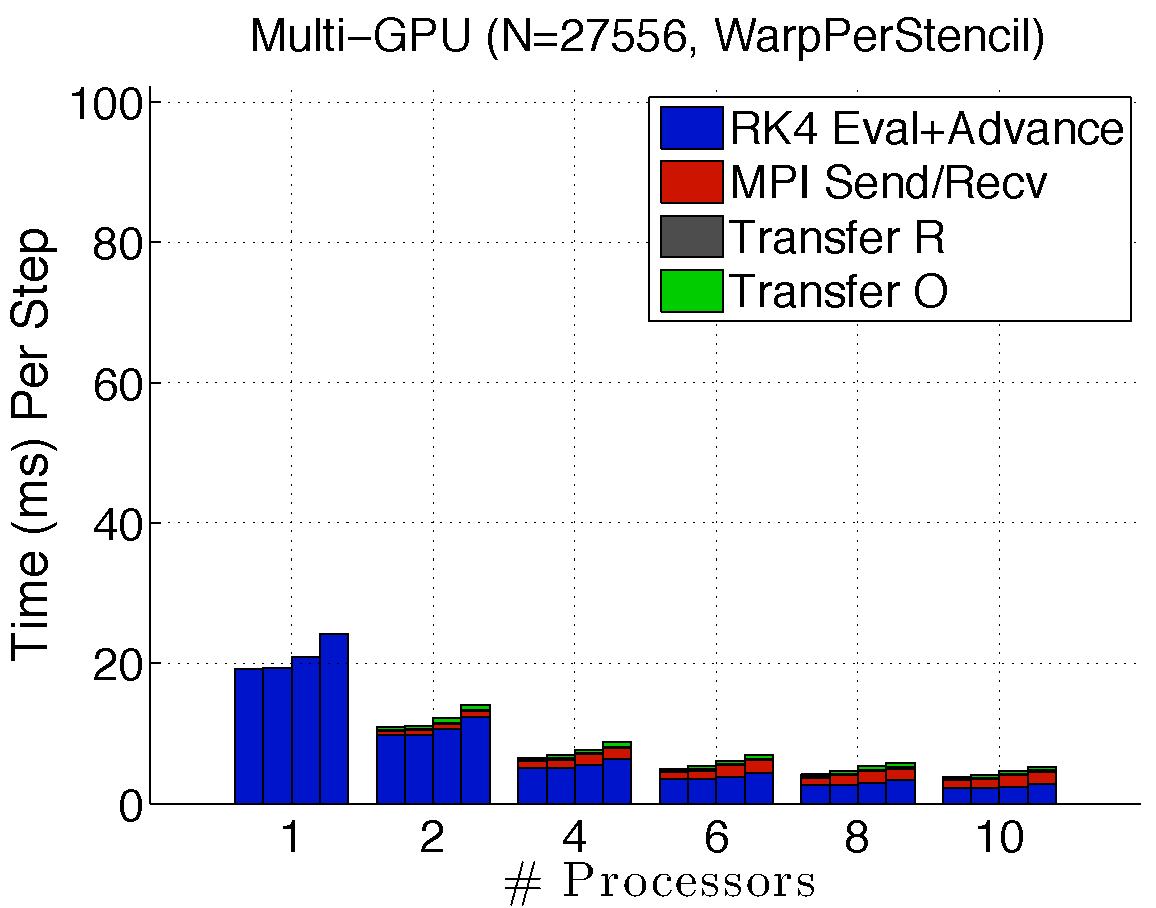
\includegraphics[width=1.0\textwidth]{../figures/chapter5/alltoallv/multiGPU_warp_costs.pdf}
\caption{Multi-GPU benchmarks by component on Keeneland}
\label{fig:alltoall_multigpu_costs}
\end{subfigure} 
\end{figure} 

Figure~\ref{fig:alltoall_1proc_warp} shows that our GPU kernel is not much different than in the paper. I have a list of optimizations I'm going through, but this test case focuses on improving the communication. 

Figure~\ref{fig:alltoall_multicpu_scaling}  shows the strong scalability of our method on Multiple CPUs. In distributed computing, ideal scaling is linear. This figure demonstrates that our method does scale linearly (almost super-linearly) as the number of CPUs increases, so our prospect for spanning all CPUs on Keeneland is within reach for problem sizes large enough. The super-linear speedup seen for 10 processors results from improved caching on processors as their individual problem sizes decrease and the processors are able to keep a larger percentage of the problem within fast cache memory.

Figure~\ref{fig:alltoall_multigpu_vs_cpu_scaling}  shows the scaling of multiple GPUs vs 1 CPU. Ideally, this figure would be the product of the previous two figures since the GPUs are attached to CPUs in a one to one correspondence. However, we see from the sub-linear scaling that while the GPU accelerators are decreasing the time to compute solutions, there is less and less return of investment as the number of processors increase. Between this Figure and the previous, the only thing that differs is the hardware on which stencils are evaluated. The cost of communication stays the same as in the previous figure. But that means the communication consumes a increasing percentage of the iteration time, until is dominates. 
Additionally, computing on the GPU requires transfer (additional communication) of data between CPU and GPU. 

Figure~\ref{fig:alltoall_multigpu_vs_gpu_scaling} shows the scalability of multiple GPUs vs 1 GPU. Here we see a sub-linear behavior for all cases. This is attributed to both the cost of transfer between CPUs and GPUs and the decreasing problem size as number of processors increases, which underutilizes the GPUs. 


Figure~\ref{fig:alltoall_multicpu_costs} and Figure~\ref{fig:alltoall_multigpu_costs} show the smaller percentage of time per iteration dedicated to communication compared to the figures in the paper. In the Figure~\ref{fig:alltoall_multigpu_costs}, the way the times bottom out indicates we are/have converged on the minimum time required to launch a GPU kernel, transfer to/from the GPU, and communicate the problem via MPI. To scale to more processors, a larger problem size is absolutely necessary.


I am generating another set of figures that demonstrate the scaling when we overlap communication and computation. MPI collectives do not allow overlap, but the asynchronous GPU kernel launches do. Therefore, I expect:
    - the scaling on multiple CPUs vs 1 CPU to be the same as it is now
    - the scaling on multiple GPUs vs 1 GPU will improve to linear/super-linear for problem sizes that occupy the hardware longer than the minimum kernel launch time. For N=27556 we might only see linear speedup up to 6 or 8 processors. 
    - larger problem sizes will still be necessary (I have benchmarks for 100K, 500K and 1M on the sphere).
    


\authnote{Need to test weak scaling (problem size stays fixed per processor). This will require a modified code, but we can fill the weight matrices with anything and run the kernels.}
\authnote{Need to compare one warp of threads to a full block of size $n$}

\section{Asynchronous OpenCL}

What are the limitations if using just async and not the queues?

\section{Multi-Queue OpenCL}
How does performance improve if we use two queues (one for Q and one for R)? 

\section{GPU Kernel Optimizations}

\subsection{Work-Group Size and Number of Stencils}
What if a work-group is larger than a warp? What if the group was occupied by multiple stencils. What improvements to speedup do we see?

How many stencils can each group handle (assuming values stay in shared memory? 
Shared memory bank conflicts? How do we sort the values? 
What is the occupancy of the GPU?

\subsection{Parallel Reduction in Shared Memory}
What significant gain do we see from adding a segmented scan to the shared memory? 

What other improvements can we think of? 

\subsection{Comparison: custom SpMV for explicit schemes vs ViennaCL}
